\documentclass[a4paper,11pt]{article}
\setlength{\headheight}{68.803pt}
\addtolength{\topmargin}{-56.803pt}

\usepackage[utf8]{inputenc}
\usepackage[T1]{fontenc}
\usepackage[italian]{babel}
\usepackage{lmodern}
\usepackage{fvextra}
\DefineVerbatimEnvironment{Verbatim}{Verbatim}{
  breaklines=true,
  breakanywhere=true,
  frame=single,
  fontsize=\small
}

% Impostazione dei margini con geometry
\usepackage[
  margin=0.72in,
  top=1.7cm,
  bottom=0.72in
]{geometry}

\usepackage[
    colorlinks=true,
    linkcolor=black,
    urlcolor=blue,
    citecolor=blue,
    pdfborder={0 0 0},
    pdfauthor={Massimo Mantineo},
    pdftitle={Progetto 1: Segmentazione clienti e Churn Prediction},
    pdfsubject={Laboratorio di Intelligenza Artificiale},
]{hyperref}

\usepackage{graphicx}
\usepackage{listings}
\usepackage{xcolor}
\usepackage{amsmath, amssymb}
\usepackage{fancyhdr}
\usepackage{setspace}
\usepackage{pgfplots}
\pgfplotsset{compat=1.17}
\usepackage{booktabs}
\usepackage{float}
\usepackage{enumitem}
\setlist{nosep, topsep=2pt, parsep=2pt}
\usepackage{caption}
\usepackage{microtype}
\usepackage{titlesec}
\titleformat{\section}{\large\bfseries}{\thesection}{1em}{}
\titleformat{\subsection}{\normalsize\bfseries}{\thesubsection}{1em}{}
\titleformat{\subsubsection}{\small\bfseries}{\thesubsubsection}{1em}{}
\titlespacing*{\section}{0pt}{10pt}{4pt}
\titlespacing*{\subsection}{0pt}{8pt}{3pt}
\titlespacing*{\subsubsection}{0pt}{6pt}{2pt}

\setlength{\footskip}{50pt}

% Impostazioni per i listing del codice Python
\lstdefinestyle{pythonstyle}{
    language=Python,
    basicstyle=\ttfamily\small,
    numbers=left,
    numberstyle=\tiny,
    stepnumber=1,
    numbersep=5pt,
    backgroundcolor=\color{white},
    showspaces=false,
    showstringspaces=false,
    showtabs=false,
    frame=single,
    tabsize=4,
    captionpos=b,
    breaklines=true,
    breakatwhitespace=true,
    keywordstyle=\color{blue}\bfseries,
    commentstyle=\color{green!50!black},
    stringstyle=\color{red},
}
\lstset{style=pythonstyle}

% Impostazione di fancyhdr per header e footer
\pagestyle{fancy}
\fancyhf{}

\fancyhead[L]{%
  \parbox[b]{0.45\textwidth}{%
    \small
    Student Name: Massimo Mantineo\\
    Student ID: 541924
    \vspace{8pt}
  }%
}
\fancyhead[C]{%
  \parbox[b]{0.2\textwidth}{%
    \centering
    \normalsize \bfseries
    Lab IA\\
    25/26
    \vspace{8pt}
  }%
}
\fancyhead[R]{%
  \parbox[b]{0.35\textwidth}{%
    \flushright
    \includegraphics[width=3.5cm]{\detokenize{logo_unime_orizontale.png}}
    \vspace{8pt}
  }%
}

\renewcommand{\contentsname}{Indice}

\begin{document}

% Pagina di copertina
\begin{titlepage}
    \thispagestyle{empty}
    \centering
    \vspace*{1cm}
    \includegraphics[width=6cm]{\detokenize{logo_unime_orizontale.png}}\par\vspace{1cm}
    \vspace{2cm}
    {\Large \textbf{Università degli Studi di Messina}\par}
    {\large Dipartimento MIFT - Corso di Laurea Triennale in Informatica (L-31)\par}
    \vspace*{1.5cm}
    {\large Laboratorio di Intelligenza Artificiale\par}
    \vspace{1.5cm}
    {\Large \textbf{PROGETTO 1:}\\
    Segmentazione Clienti e Churn Prediction\par}
    \vspace{2.5cm}
    {\large Massimo Mantineo \par}
    {\large Matricola: 541924 \par}
    \vfill
    {\large Messina, A.A. 2025/2026 \par}
\end{titlepage}

\clearpage
\pagestyle{fancy}
% \tableofcontents
% \vspace{0.8cm}

\begin{abstract}
In questo progetto ho studiato come unire il clustering (apprendimento non supervisionato) e la classificazione (apprendimento supervisionato) per analizzare il comportamento dei clienti di una compagnia telefonica (usando il dataset Telco Customer Churn). L'obiettivo principale è prevedere quali clienti rischiano di abbandonare l'operatore (churn prediction). Prima ho diviso i clienti in due gruppi (cluster) con l'algoritmo k-Means, trovando un profilo di clienti fedeli che spendono poco e uno di clienti a rischio che spendono molto. Poi ho addestrano tre modelli per la classificazione: la Regressione Logistica, un Albero di Decisione e una Rete Neurale (MLP). Ho confrontato le prestazioni dei modelli con e senza la feature del cluster. La Regressione Logistica e l'Albero hanno mostrato prestazioni stabili (~80.6\% accuratezza), mentre la rete neurale MLP ha avuto un forte overfitting. Tuttavia, aggiungendo il cluster come feature, la Recall (cioè la capacità di individuare chi abbandona davvero) dell'MLP sul test set è salita dal 42.8\% al 58.3\% (+15.5\%). Nelle conclusioni discuto l'interpretabilità dei modelli, i loro limiti e le possibili migliorie come il bilanciamento dei dati.
\end{abstract}
\vspace{0.4cm}

% -------------------------------------------------------------
\section{Descrizione del problema}
\label{sec:descrizione_problema}
Per un'azienda telefonica, perdere un cliente (fenomeno chiamato \textit{customer churn} o abbandono) è un grosso problema economico. Trovare nuovi clienti costa molto più che tenersi quelli già attivi. Per questo è utile costruire un sistema che possa prevedere in anticipo se un cliente sta per andarsene, in modo che l'azienda possa fargli un'offerta e convincerlo a restare.

Questo progetto affronta il problema usando due approcci del Machine Learning in una pipeline integrata: il clustering (non supervisionato) e la classificazione (supervisionata).

\subsection{Il Task Non Supervisionato (Clustering)}
Con il clustering vogliamo dividere i clienti in gruppi (o segmenti) in base a quanto si somigliano nei loro comportamenti (costi, tipo di contratto, mesi di permanenza). L'apprendimento è ``non supervisionato'' perché il computer fa questa divisione da solo, senza sapere in anticipo chi ha abbandonato o meno la compagnia.

La segmentazione dei clienti viene qui affrontata con l'algoritmo $k$-Means, provando a dividere i clienti in 2, 3 o 4 gruppi. Per scegliere il numero migliore di gruppi uso due indicatori:
\begin{itemize}
    \item \textbf{Inertia (Metodo del Gomito)}: misura quanto i punti sono vicini al centro del proprio gruppo. Più il valore è basso, più i gruppi sono compatti internamente.
    \item \textbf{Silhouette Score}: misura quanto un cliente è simile al proprio gruppo rispetto a quanto sia dissimile dagli altri. Varia tra -1 e +1; valori più alti indicano gruppi ben separati e definiti.
\end{itemize}

\subsection{Il Task Supervisionato (Classificazione)}
Il secondo compito è una classificazione binaria. Vogliamo addestrare un modello che, guardando le caratteristiche di un cliente (come contratti, costi e il gruppo in cui è stato inserito), riesca a prevedere se abbandonerà la compagnia (classe $1$, \textit{Churn: Sì}) o rimarrà fedele (classe $0$, \textit{Churn: No}).

\subsection{Le Metriche di Valutazione della Classificazione}
Per capire se i modelli funzionano bene, ho usato tre metriche classiche:
\begin{itemize}
    \item \textbf{Accuracy (Accuratezza)}: ci dice semplicemente quante predizioni sono corrette sul totale delle prove.
    \begin{equation}
        \text{Accuracy} = \frac{TP + TN}{TP + TN + FP + FN}
    \end{equation}
    dove i singoli elementi rappresentano:
    \begin{itemize}
        \item $TP$ (\textit{True Positives} - Veri Positivi): Clienti che volevano andarsene e che il modello ha identificato correttamente come in partenza.
        \item $TN$ (\textit{True Negatives} - Veri Negativi): Clienti fedeli che il modello ha correttamente identificato come stabili.
        \item $FP$ (\textit{False Positives} - Falsi Positivi): Clienti fedeli che il modello ha erroneamente previsto come in partenza.
        \item $FN$ (\textit{False Negatives} - Falsi Negativi): Clienti in partenza che il modello ha erroneamente previsto come stabili.
    \end{itemize}
    In parole semplici, l'Accuratezza è il rapporto tra tutte le risposte esatte del modello (sia per chi resta, sia per chi va via) e il numero totale di clienti analizzati. Rappresenta la percentuale di successo complessiva, ma può essere ingannevole se le classi sono sbilanciate.
    \item \textbf{Recall (Richiamo)}: ci dice quanti dei clienti che vogliono abbandonare davvero vengono scoperti dal modello:
    \begin{equation}
        \text{Recall} = \frac{TP}{TP + FN}
    \end{equation}
    Conceptualizzando questa formula, il denominatore ($TP + FN$) rappresenta la totalità dei clienti che stanno effettivamente abbandonando la compagnia. La Recall ci dice quindi quale percentuale di questa "lista rossa" il nostro modello è stato in grado di intercettare. Nel nostro caso, questa è la metrica più importante per il business: se il modello commette un falso negativo ($FN$), l'azienda perde il cliente senza avergli potuto proporre offerte di fidelizzazione.
    \item \textbf{AUC (Area Under the ROC Curve)}: misura la capacità del modello di distinguere tra le due classi a prescindere dalla soglia di decisione scelta. Varia tra $0.5$ (scelte del tutto casuali, come lanciare una moneta) e $1.0$ (modello perfetto che non sbaglia mai). È una misura molto robusta quando le classi sono sbilanciate.
\end{itemize}

% -------------------------------------------------------------
\section{Dataset e preparazione dei dati}
\label{sec:dataset_preparazione}
Ho utilizzato il dataset reale \textit{Telco Customer Churn} fornito storicamente da IBM. Non si tratta di una risorsa qualsiasi reperita casualmente sul web, ma di un dataset di riferimento (benchmark standard) ampiamente studiato nella comunità di Machine Learning per problemi di retention dei clienti. In totale contiene $7043$ clienti di una compagnia di telecomunicazioni, descritti da $21$ variabili (colonne) che coprono i loro dati anagrafiche, i servizi sottoscritti (fibra, telefono, streaming) e il loro stato di fedeltà.

\subsection{Struttura e Principali Variabili}
Le caratteristiche si dividono in tre categorie principali:
\begin{enumerate}
    \item \textbf{Variabili numeriche continue}: mesi da cui il cliente è attivo (\textit{tenure}), spesa mensile (\textit{MonthlyCharges}) e spesa totale (\textit{TotalCharges}).
    \item \textbf{Variabili categoriche qualitative}: tipo di contratto (\textit{Contract}: mensile, annuale, biennale), metodo di pagamento (\textit{PaymentMethod}), tipo di connessione internet (\textit{InternetService}) e altri servizi accessori (es. backup online, streaming tv).
    \item \textbf{Variabili categoriche binarie (sì/no)}: genere, se ha un partner o familiari a carico, se usa la bolletta online e se è un cliente anziano (\textit{SeniorCitizen}, codificata numericamente in $\{0, 1\}$).
\end{enumerate}
La variabile da prevedere è \textbf{Churn}, che assume valore ``Yes'' se il cliente ha abbandonato la compagnia nell'ultimo mese, ``No'' in caso contrario.

Durante l'analisi iniziale emerge un'anomalia nella variabile \textit{TotalCharges}. Sebbene indichi costi totali monetari, il suo tipo in Python viene rilevato come testo (\texttt{object}) anziché numerico. Questa anomalia è dovuta alla presenza di $11$ righe che contengono spazi vuoti (\texttt{" "}). Incrociando questi dati, si nota che questi record corrispondono a nuovi clienti registrati da zero mesi (\texttt{tenure = 0}), per i quali la spesa complessiva è effettivamente pari a zero. Python interpreta gli spazi vuoti come stringhe, impedendo qualsiasi operazione matematica: nel preprocessing dovremo sostituire questi spazi vuoti con \texttt{0.0} e convertire la colonna in formato numerico.

\subsection{Operazioni di Preprocessing e Risposte Metodologiche}
Prima di addestrare i modelli ho dovuto sistemare e preparare i dati con alcuni passaggi fondamentali.

\subsubsection{Gestione dei valori mancanti e Imputazione}
Nella colonna \textit{TotalCharges} c'erano 11 righe con spazi vuoti. Andando a controllare, ho notato che tutti questi clienti avevano \textit{tenure} pari a $0$ mesi (erano clienti appena registrati che non avevano ancora ricevuto nessuna bolletta). Per questo motivo, invece di cancellarli o usare valori calcolati, ho scelto di inserire semplicemente \texttt{0.0}.

\textbf{Che cos'è l'imputazione con la mediana e come si calcola?}\\
Se avessimo voluto riempire i dati mancanti usando la mediana, avremmo ordinato tutti i valori dal più piccolo al più grande e preso quello centrale (o la media dei due centrali se il numero totale è pari).

Matematicamente, per calcolare il valore mediano:
1. Si ordinano gli $N$ valori della variabile in ordine non decrescente: $x_1 \leq x_2 \leq \dots \leq x_N$.
2. Se $N$ è dispari, la mediana è il valore centrale in posizione $\frac{N+1}{2}$:
\begin{equation}
    \text{Mediana} = x_{\frac{N+1}{2}}
\end{equation}
3. Se $N$ è pari, la mediana è la media aritmetica dei due valori centrali in posizione $\frac{N}{2}$ e $\frac{N}{2}+1$:
\begin{equation}
    \text{Mediana} = \frac{x_{\frac{N}{2}} + x_{\frac{N}{2}+1}}{2}
\end{equation}

\textbf{Esempio pratico per capire le formule:}
\begin{itemize}
    \item \textbf{Caso Dispari ($N=5$)}: se abbiamo i valori ordinati $\{10, 20, 30, 40, 50\}$, la formula ci dice di prendere il valore alla posizione $\frac{5+1}{2} = 3$, che corrisponde a $30$.
    \item \textbf{Caso Pari ($N=6$)}: se abbiamo i valori ordinati $\{10, 20, 30, 40, 50, 60\}$, i due valori centrali sono in posizione $\frac{6}{2}=3$ (ovvero $30$) e in posizione $\frac{6}{2}+1=4$ (ovvero $40$). Facciamo la loro media aritmetica: $\frac{30+40}{2} = 35$.
\end{itemize}

\textbf{Perché si usa la mediana invece della media?}\\
La mediana è ottima perché è robusta contro i valori estremi (outlier), a differenza della media che risente pesantemente di un singolo valore molto alto o molto basso. Nel nostro caso, però, mettere \texttt{0.0} era la scelta logicamente corretta per il business, mentre usare la mediana generale (circa $1397.47\$$) sarebbe stato un errore perché avrebbe assegnato una spesa alta a persone che non sono ancora clienti da un mese.

\subsubsection{Codifica delle variabili categoriche (One-Hot Encoding)}
I modelli matematici non capiscono le parole (come ``Mensile'' o ``Annuale''). Perciò ho usato il One-Hot Encoding:
\begin{itemize}
    \item \textbf{In cosa consiste?}\\
    Consiste nel mappare una variabile qualitativa con $C$ categorie distinte in $C$ variabili binarie (aventi valore $1$ se l'osservazione appartiene alla categoria e $0$ altrimenti).
    \item \textbf{Perché escludiamo una categoria (drop\_first=True)?}\\
    Per evitare problemi matematici (multicollinearità). Se tenessimo tutte le $C$ colonne, la loro somma darebbe sempre $1$, creando una dipendenza lineare perfetta con il termine di intercetta (bias) dei modelli lineari, il che rende impossibile invertire le matrici nei calcoli. Escludendo la prima colonna, questa funge da riferimento. Ad esempio, per il tipo di contratto (mensile, annuale, biennale), bastano due colonne (annuale e biennale): se entrambe sono 0, significa che il contratto è mensile.
    \item \textbf{Come verifichiamo la correttezza nel codice?}\\
    Ho usato la funzione \texttt{pd.get\_dummies()} di pandas. Per verificare:
    \begin{enumerate}
        \item Ho controllato le dimensioni della tabella (il numero di colonne è passato da 20 a 30).
        \item Ho guardato le prime righe per verificare che ci fossero solo 0 e 1 nelle nuove colonne.
    \end{enumerate}
\end{itemize}

\subsubsection{Standardizzazione (Standard Scaling)}
I modelli basati sulle distanze ($k$-Means) e sulle reti neurali (MLP) risentono fortemente delle differenze di scala tra le variabili.
\begin{itemize}
    \item \textbf{Come funziona lo Standard Scaling e cosa significano i simboli?}\\
    La standardizzazione trasforma le variabili numeriche in modo che abbiano tutte lo stesso intervallo d'azione. Per ciascun valore $x_i$, si calcola il valore scalato $z_i$ tramite la formula:
    \begin{equation}
        z_i = \frac{x_i - \mu}{\sigma}
    \end{equation}
    dove i componenti matematici sono:
    \begin{itemize}
        \item \textbf{La Media ($\mu$)}: Rappresenta il baricentro o valore medio aritmetico. Si sommano tutti gli $N$ valori e si divide per $N$:
        \begin{equation}
            \mu = \frac{1}{N}\sum_{i=1}^{N} x_i
        \end{equation}
        \item \textbf{La Deviazione Standard ($\sigma$)}: Rappresenta quanto, in media, i singoli valori si discostano dal valore medio. Se i dati sono molto dispersi (es. spese da 10\$ a 1000\$), $\sigma$ sarà grande; se sono tutti concentrati, $\sigma$ sarà piccola:
        \begin{equation}
            \sigma = \sqrt{\frac{1}{N}\sum_{i=1}^{N} (x_i - \mu)^2}
        \end{equation}
    \end{itemize}
    In parole semplici, sottraendo la media $\mu$ al numeratore si sposta il centro dei dati a $0$. Dividendo poi per $\sigma$, si fa in modo che l'unità di misura diventi "quante deviazioni standard dista questo punto dal centro". In questo modo, variabili con range enormi (come la spesa totale, da 0 a 8000\$) e variabili con range ristretti (come i mesi di permanenza, da 0 a 72) vengono portate sulla stessa identica scala numerica, evitando che il costo totale schiacci l'importanza della durata del contratto.
    \item \textbf{Perché lo splitting in Train/Test si fa PRIMA dello scaling?}\\
    Questa è una regola fondamentale per evitare il \textbf{Data Leakage} (trapelamento di informazioni). Se calcolassimo la media $\mu$ e la deviazione standard $\sigma$ su tutto il dataset prima di dividerlo, le informazioni del test set (che deve simulare dati futuri sconosciuti) influenzerebbero i valori del train set. Perciò ho diviso prima il dataset, calcolato i parametri di scaling solo sul Train, e infine li ho applicati a entrambi.
\end{itemize}

\begin{figure}[htbp]
    \centering
    \begin{minipage}{0.48\textwidth}
        \centering
        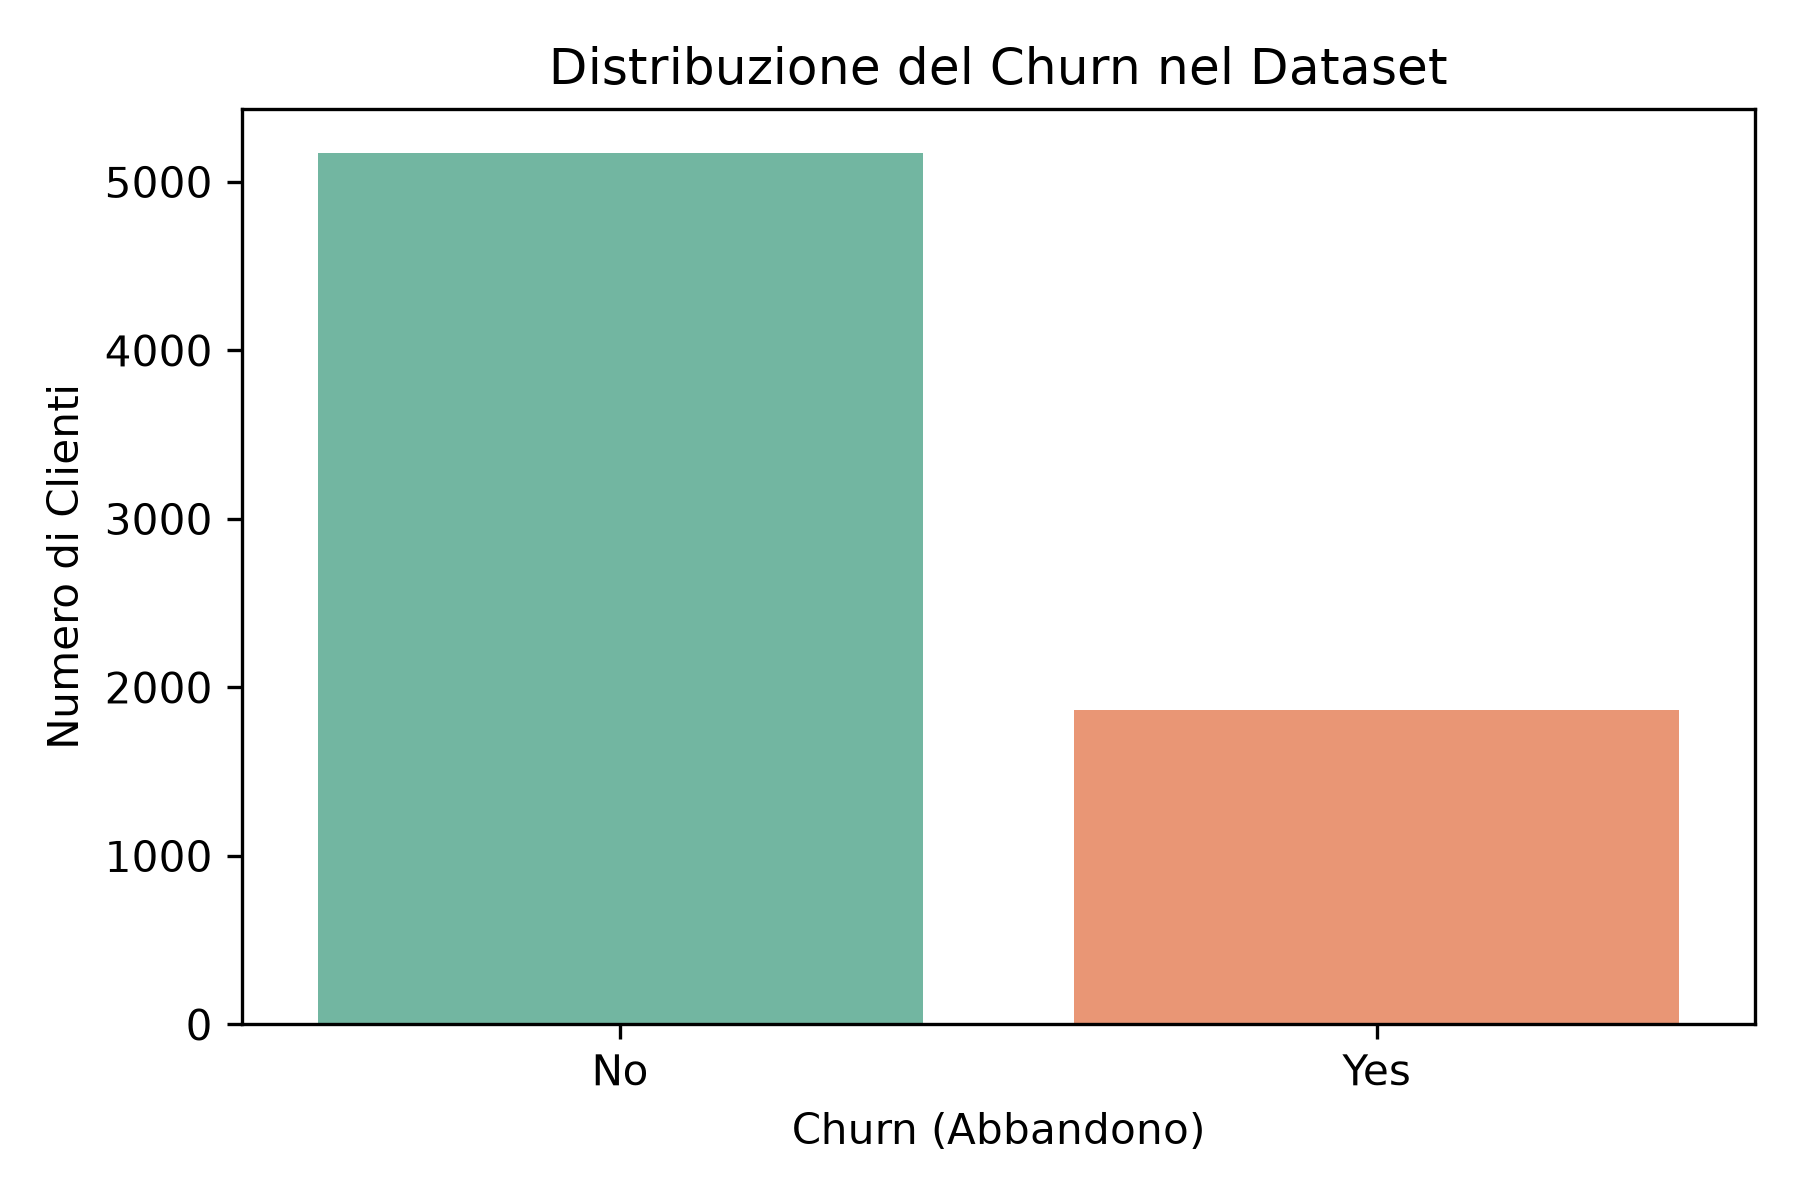
\includegraphics[width=\textwidth]{../grafici/churn_distribution.png}
        \caption{Distribuzione del Churn nel dataset.}
        \label{fig:churn_dist}
    \end{minipage}\hfill
    \begin{minipage}{0.48\textwidth}
        \centering
        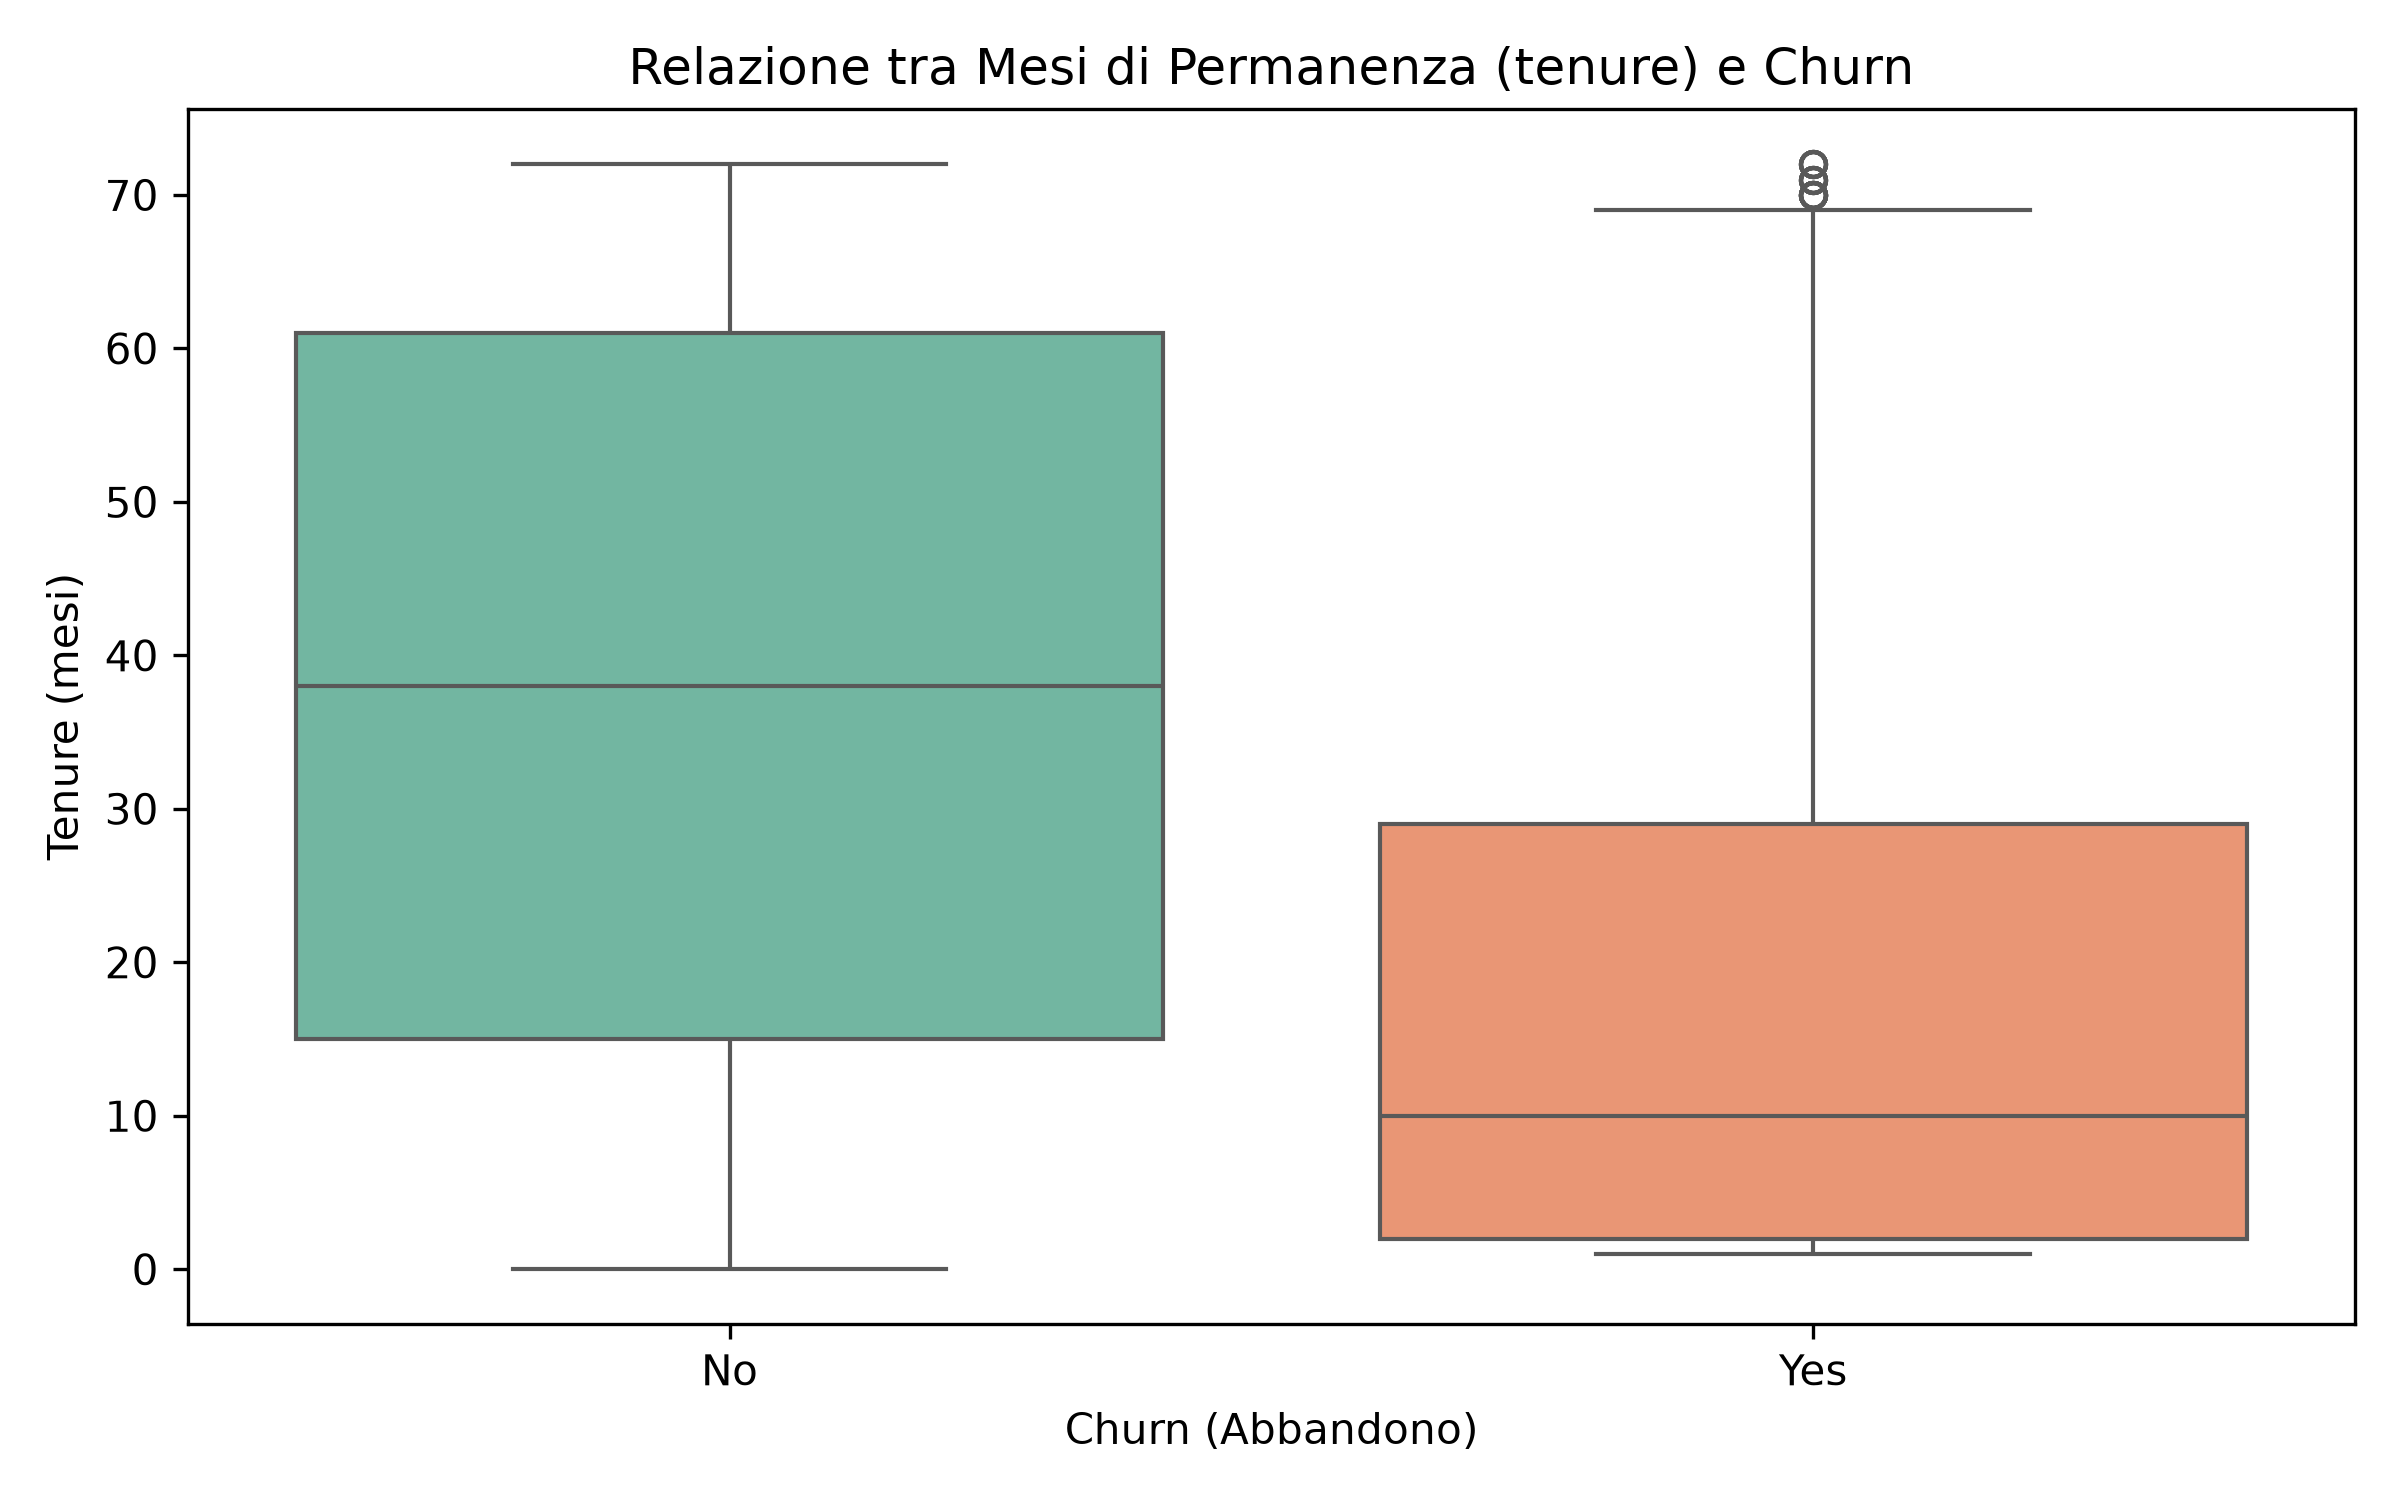
\includegraphics[width=\textwidth]{../grafici/churn_vs_tenure.png}
        \caption{Relazione tra mesi di permanenza (tenure) e Churn.}
        \label{fig:churn_tenure}
    \end{minipage}
\end{figure}

\subsection{Criticità: Sbilanciamento delle Classi e Interpretazione dei Grafici}
Analizzando i due grafici sopra:
\begin{enumerate}
    \item \textbf{Distribuzione del Churn (Figura \ref{fig:churn_dist})}: Il dataset presenta una chiara sproporzione delle classi: $5174$ clienti ($73.4\%$) appartengono alla classe ``No Churn'' (classe 0) e solo $1869$ ($26.6\%$) alla classe ``Yes Churn'' (classe 1). Questo sbilanciamento (rapporto 3:1) è una forte criticità: se un modello banale dicesse sempre 'No Churn', avrebbe un'accuratezza del $73.4\%$. Per proteggere la validità dei test, ho applicato uno split train-test stratificato, preservando la proporzione del $26.6\%$ di Churn in entrambi i set.
    \item \textbf{Relazione tra Churn e Mesi (Figura \ref{fig:churn_tenure})}: Il boxplot evidenzia la distribuzione del numero di mesi di permanenza dei clienti. Per chi ha abbandonato la compagnia (Yes Churn), la scatola è fortemente compressa verso il basso, con una mediana di circa 10 mesi. Significa che la maggior parte di chi abbandona è cliente da meno di un anno. Al contrario, la scatola di chi rimane fedele (No Churn) è posizionata molto più in alto, con una mediana di circa 38 mesi, confermando che i clienti storici sono molto più stabili.
\end{enumerate}

% -------------------------------------------------------------
\section{Metodologia}
\label{sec:metodologia}
La mia pipeline di lavoro è divisa in tre parti:
1. Pulizia dei dati, codifica delle categoriche e standardizzazione.
2. Applicazione di $k$-Means per generare la feature del cluster e aggiunta di questa colonna al dataset.
3. Addestramento dei tre classificatori (Regressione Logistica, Albero di Decisione, MLP) sia con che senza la colonna del cluster, per valutarne l'effetto.

\subsection{I Modelli Scelti}

\subsubsection{k-Means (Clustering)}
L'algoritmo $k$-Means serve a dividere i dati in gruppi. All'inizio sceglie a caso dei punti centrali (centroidi) per ogni gruppo. Poi ripete due passi:
\begin{enumerate}
    \item Assegna ogni cliente al gruppo il cui centroide è più vicino (usando la distanza euclidea).
    \item Ricalcola il centro di ogni gruppo facendo la media delle posizioni dei punti assegnati ad esso.
\end{enumerate}
Si ferma quando i centri non si muovono più. Ho provato soluzioni con 2, 3 e 4 cluster valutando Inertia e Silhouette Score per scegliere il numero ottimale di gruppi.

\subsubsection{Regressione Logistica (Baseline)}
Usata come baseline semplice. Calcola una somma pesata delle caratteristiche del cliente (in cui ciascuna variabile ha un peso che ne determina l'importanza) e passa questo punteggio lineare, che chiamiamo $t$, all'interno della funzione \textbf{Sigmoide}:
\begin{equation}
    \sigma(t) = \frac{1}{1 + e^{-t}}
\end{equation}
dove $e$ è il numero di Eulero (una costante matematica fondamentale pari a circa $2.718$).

\textbf{Spiegazione intuitiva del funzionamento:}
\begin{itemize}
    \item Se il cliente ha indizi molto forti di fedeltà, il punteggio pesato $t$ sarà un numero negativo molto grande (es. $t = -5$). La formula diventa $\sigma(-5) = \frac{1}{1 + e^5} \approx \frac{1}{1 + 148} \approx 0.006$, indicando uno $0.6\%$ di probabilità di abbandono (il cliente è sicuro).
    \item Se il cliente mostra un comportamento tipico di chi sta per andarsene, il punteggio $t$ sarà un numero positivo molto grande (es. $t = 5$). La formula diventa $\sigma(5) = \frac{1}{1 + e^{-5}} \approx \frac{1}{1 + 0.0067} \approx 0.993$, indicando una probabilità del $99.3\%$ di abbandono.
    \item Se la situazione è di massima incertezza, il punteggio è $t = 0$, e la formula restituisce $\sigma(0) = \frac{1}{1+1} = 0.5$ (probabilità del $50\%$).
\end{itemize}
In sintesi, questa funzione a forma di ``S'' (curva logistica) serve a comprimere qualsiasi valore numerico in un intervallo stretto tra 0 e 1, permettendoci di leggerlo direttamente come una probabilità di Churn.

\subsubsection{Decision Tree (Modello Principale 1)}
Questo modello ragiona a domande sì/no (regole). Sceglie le suddivisioni migliori per separare il più possibile i clienti a rischio da quelli fedeli, misurando la purità dei gruppi tramite l'indice di Gini. Ho impostato la profondità massima dell'albero a $5$ (\texttt{max\_depth=5}) per evitare che cresca troppo e impari a memoria le risposte (overfitting).

\subsubsection{Multi-Layer Perceptron (Modello Principale 2)}
Il Multi-Layer Perceptron (MLP) è una rete neurale artificiale composta da vari strati di neuroni collegati tra loro.

L'addestramento funziona in due fasi ripetute iterativamente:
\begin{enumerate}
    \item \textbf{Fase in avanti (Forward Propagation)}: I dati del cliente entrano nella rete, passano per gli strati nascosti (dove i neuroni calcolano somme pesate e applicano una funzione di attivazione non lineare come la ReLU, $f(x) = \max(0, x)$) e arrivano all'uscita.
    \item \textbf{Fase all'indietro (Backpropagation)}: Si calcola l'errore tra la risposta della rete e quella reale (usando la perdita di cross-entropia). L'errore viene propagato a ritroso per correggere i pesi dei collegamenti usando un ottimizzatore (Adam) basato sulla discesa del gradiente.
\end{enumerate}

\textbf{Spiegazione intuitiva delle funzioni di attivazione:}
\begin{itemize}
    \item \textbf{La ReLU ($f(x) = \max(0, x)$) negli strati nascosti}: Se il segnale in ingresso $x$ è negativo o debole, la funzione restituisce $0$ (il neurone rimane spento); se è positivo, lo lascia passare invariato. Funge in pratica da interruttore biologico, consentendo alla rete di attivare percorsi diversi in base ai dati e di apprendere relazioni non lineari complesse.
    \item \textbf{La Sigmoide nello strato di uscita}: Viene utilizzata alla fine per lo stesso motivo descritto per la Regressione Logistica: schiacciare il valore reale finale calcolato dalla rete in una probabilità comprensibile tra 0 e 1.
\end{itemize}

\textbf{Perché nei neuroni nascosti servono funzioni non lineari?}\\
Senza di esse, la composizione di più strati lineari collasserebbe matematicamente in una singola trasformazione lineare. La rete neurale perderebbe così la capacità di apprendere relazioni complesse, diventando equivalente ad un semplice modello di Regressione Logistica.

\subsection{Riproducibilità, Dipendenze e Istruzioni d'Esecuzione}
Per rendere il progetto riproducibile, tutto il codice --- comprendente l'analisi esplorativa dei dati, il preprocessing, la segmentazione tramite clustering ed i modelli di classificazione --- è interamente implementato e documentato all'interno del Jupyter Notebook \texttt{segmentazione\_crunch.ipynb} situato nella cartella \texttt{codice/}. Se il dataset non è presente localmente nella cartella \texttt{dati/}, il notebook provvede a scaricarlo automaticamente all'avvio.

Le librerie usate con le rispettive versioni di riferimento sono:
\begin{itemize}
    \item \textbf{Pandas} e \textbf{NumPy} per gestire le tabelle e i calcoli matematici.
    \item \textbf{Scikit-Learn} per il clustering ($k$-Means) e i modelli di classificazione.
    \item \textbf{Matplotlib} e \textbf{Seaborn} per disegnare i grafici.
\end{itemize}
Le dipendenze esatte sono raccolte nel file \texttt{requirements.txt} e le istruzioni di installazione sono spiegate nel file \texttt{README.md} nella radice del progetto.

\subsection{Setup Sperimentale e Prevenzione di Overfitting e Underfitting}
Per valutare l'affidabilità dei modelli, dobbiamo monitorare attentamente due possibili comportamenti problematici:
\begin{itemize}
    \item \textbf{Overfitting (imparare a memoria)}: Si verifica quando un modello apprende eccessivamente i dettagli e il rumore del Training Set, perdendo capacità di generalizzazione su dati nuovi (Test Set). Si riconosce quando le metriche sul Train sono quasi perfette, ma crollano sul Test.
    \item \textbf{Underfitting (troppo semplice)}: Si verifica quando il modello è troppo semplice per catturare la struttura fondamentale dei dati. Si riconosce quando le metriche sono scarse sia sul Training Set che sul Test Set.
\end{itemize}
Nel nostro esperimento, addestriamo i modelli sull'80\% dei dati (Train, stratificato per mantenere la proporzione di churn) e li valutiamo sul restante 20\% (Test). Monitoriamo l'underfitting verificando che la baseline (Regressione Logistica) e l'albero di decisione raggiungano almeno l'80\% di accuratezza sul train (confermando che hanno appreso le regole di base), e monitoriamo l'overfitting controllando il divario tra train e test.

\subsection{Caratterizzazione dei due Cluster ($k=2$)}
Dopo aver eseguito l'algoritmo k-Means con $k=2$, ho analizzato le caratteristiche dei clienti nei due gruppi (usando i valori originali prima della standardizzazione):
\begin{enumerate}
    \item \textbf{Cluster 0 (1526 clienti - ``Fedeli e con spesa bassa'')}:
    \begin{itemize}
        \item Tenure media: $30.55$ mesi.
        \item Spesa mensile media (\textit{MonthlyCharges}): $21.08\$$.
        \item Costo totale medio (\textit{TotalCharges}): $662.60\$$.
        \item Tasso di Churn reale: \textbf{7.40\%} (estremamente basso).
        \item Contratti: Prevalenza di contratti a lungo termine (Biennali: $41.8\%$, Annuali: $23.9\%$, Mensili: $34.3\%$).
        \item \textit{Profilo}: Clientela stabile che utilizza servizi di base, caratterizzata da elevata fedeltà e contratti pluriennali.
    \end{itemize}
    \item \textbf{Cluster 1 (5517 clienti - ``A rischio e con spesa alta'')}:
    \begin{itemize}
        \item Tenure media: $32.88$ mesi.
        \item Spesa mensile media (\textit{MonthlyCharges}): $76.84\$$.
        \item Costo totale medio (\textit{TotalCharges}): $2727.03\$$.
        \item Tasso di Churn reale: \textbf{31.83\%} (molto alto).
        \item Contratti: Forte prevalenza di contratti flessibili mensili (Mese-a-mese: $60.7\%$).
        \item \textit{Profilo}: Clientela ad alto consumo tecnologico (banda larga, streaming), ma molto volatile e legata a contratti mensili senza vincoli temporali.
    \end{itemize}
\end{enumerate}

% -------------------------------------------------------------
\section{Risultati e Interpretazione}
\label{sec:risultati}

\subsection{Risultati del Clustering k-Means}
Ho testato k-Means con 2, 3 e 4 cluster. I risultati di Inertia e Silhouette Score sono riportati nella Tabella \ref{tab:clustering_metrics}.

\begin{table}[htbp]
\centering
\caption{Metriche di valutazione del clustering k-Means.}
\label{tab:clustering_metrics}
\begin{tabular}{ccc}
\toprule
\textbf{Numero di Cluster ($k$)} & \textbf{Inertia} & \textbf{Silhouette Score} \\
\midrule
2 & 41817.82 & 0.2946 \\
3 & 30802.81 & 0.2861 \\
4 & 28228.08 & 0.2279 \\
\bottomrule
\end{tabular}
\end{table}

La Figura \ref{fig:clustering_eval} mostra l'andamento congiunto dell'Inertia (curva rossa) e del Silhouette Score (curva blu):
\begin{itemize}
    \item \textbf{Inertia}: Mostra una discesa rapida e un cambio di pendenza (il ``gomito'') a $k=2$ e $k=3$.
    \item \textbf{Silhouette Score}: Raggiunge il suo massimo assoluto proprio a $k=2$ ($0.2946$) e poi decresce per $k=3$ e $k=4$.
\end{itemize}
Questi indicatori indicano che la scelta ottimale è \textbf{k=2}, in quanto garantisce la massima separazione e coesione dei gruppi, fornendo al contempo profili commerciali chiari e facilmente interpretabili per le strategie di business. La visualizzazione spaziale di questa suddivisione a due cluster è illustrata nella mappa di clustering (Figura \ref{fig:clustering_map}), dove si osserva graficamente la netta separazione tra i due gruppi di clienti.

\begin{figure}[htbp]
    \centering
    \begin{minipage}{0.48\textwidth}
        \centering
        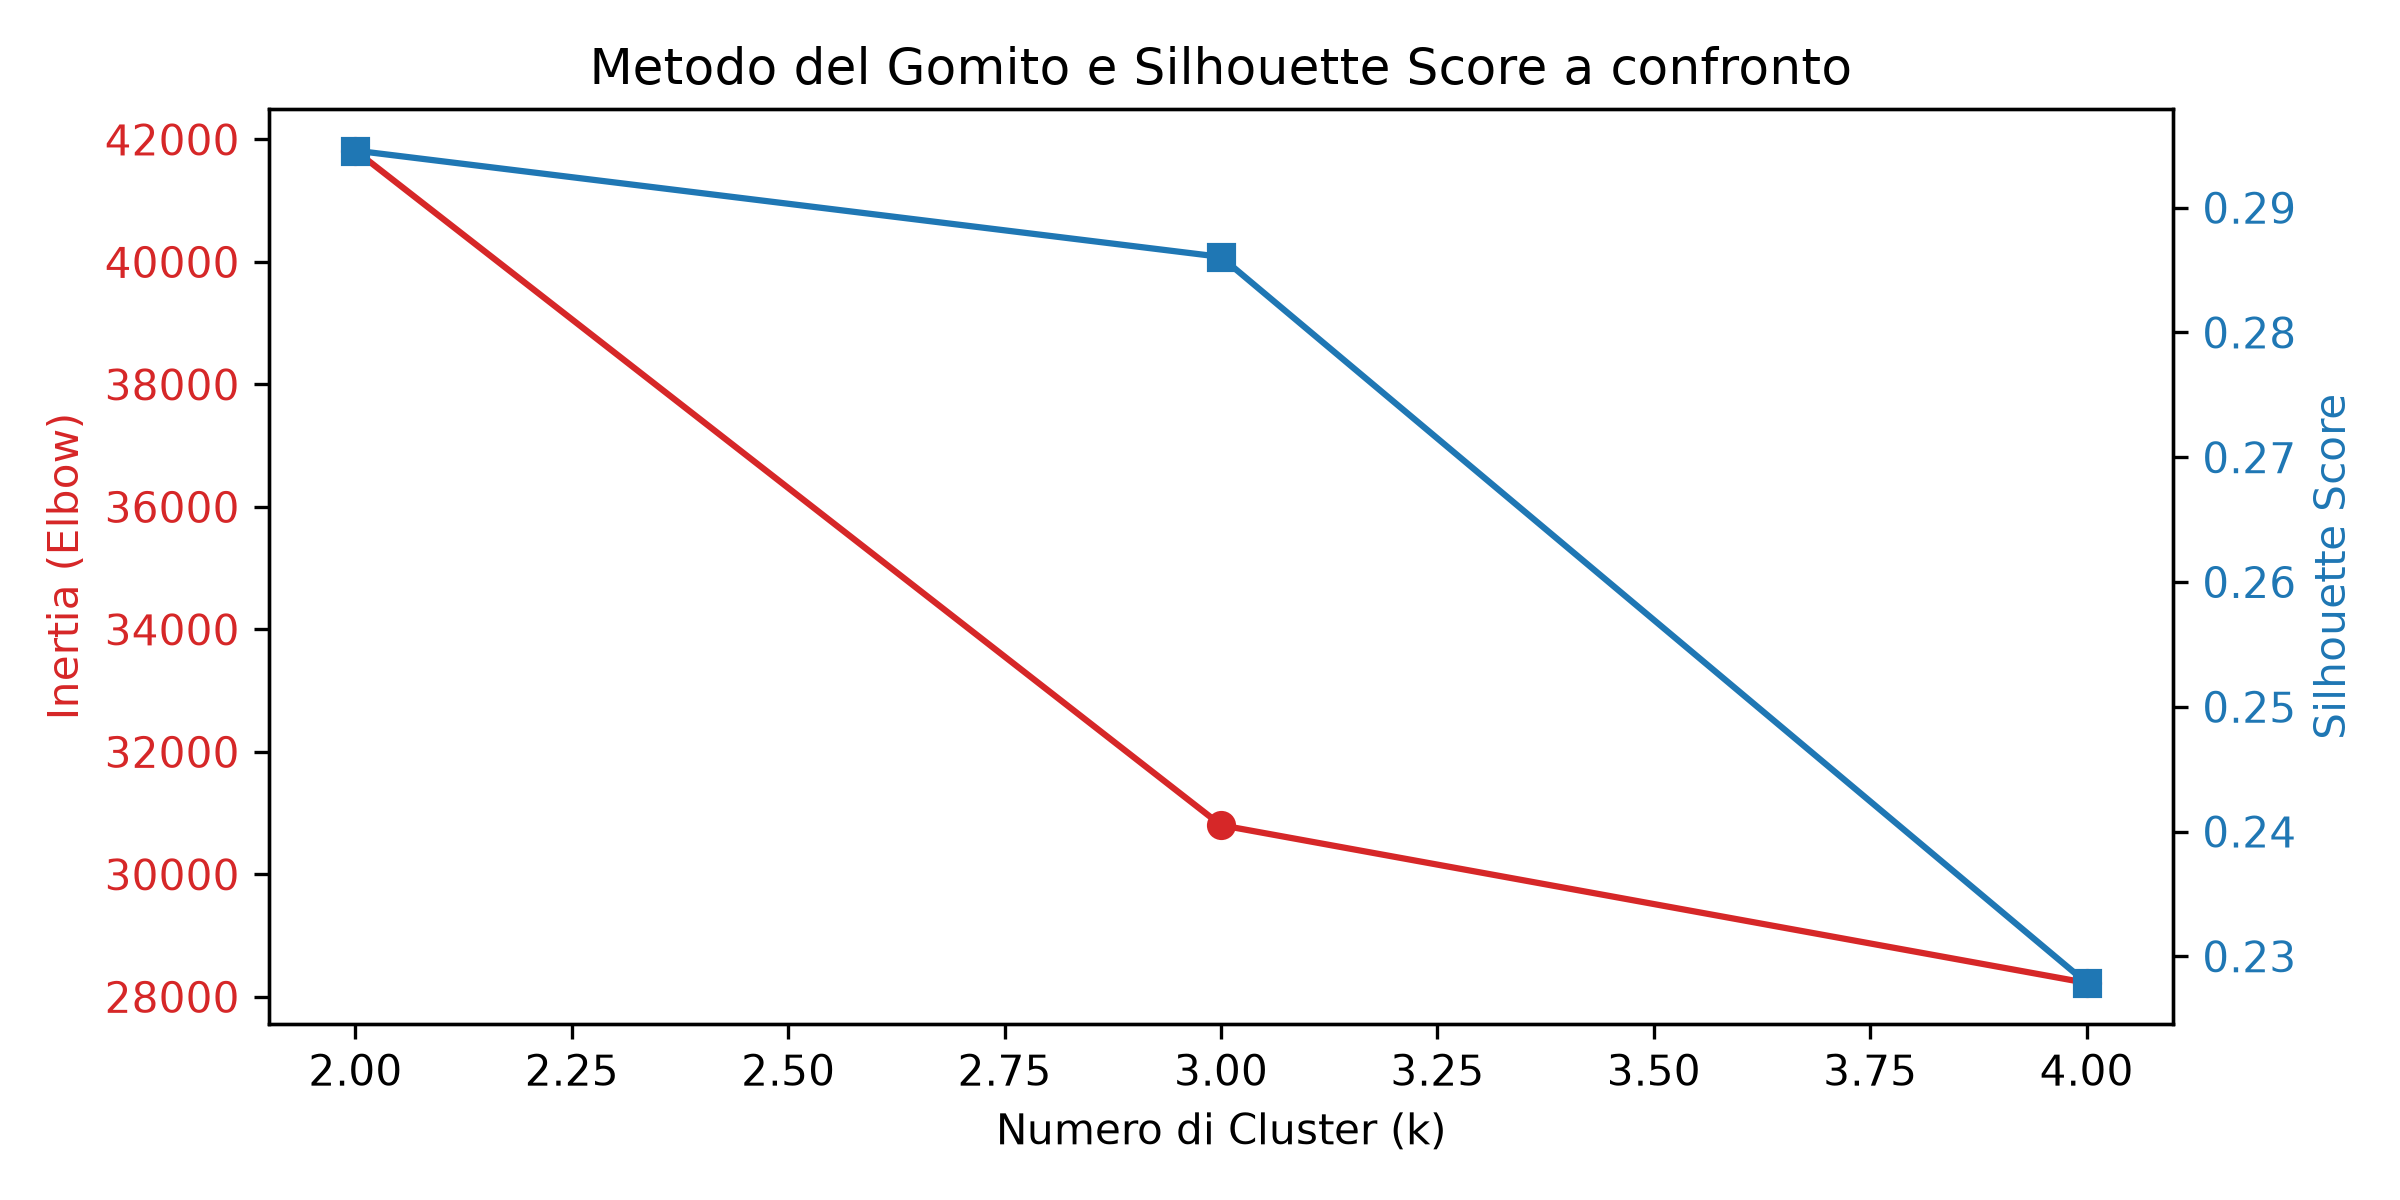
\includegraphics[width=\textwidth]{../grafici/clustering_evaluation.png}
        \caption{Valutazione del clustering k-Means tramite metodo del gomito (Inertia) e Silhouette Score.}
        \label{fig:clustering_eval}
    \end{minipage}\hfill
    \begin{minipage}{0.48\textwidth}
        \centering
        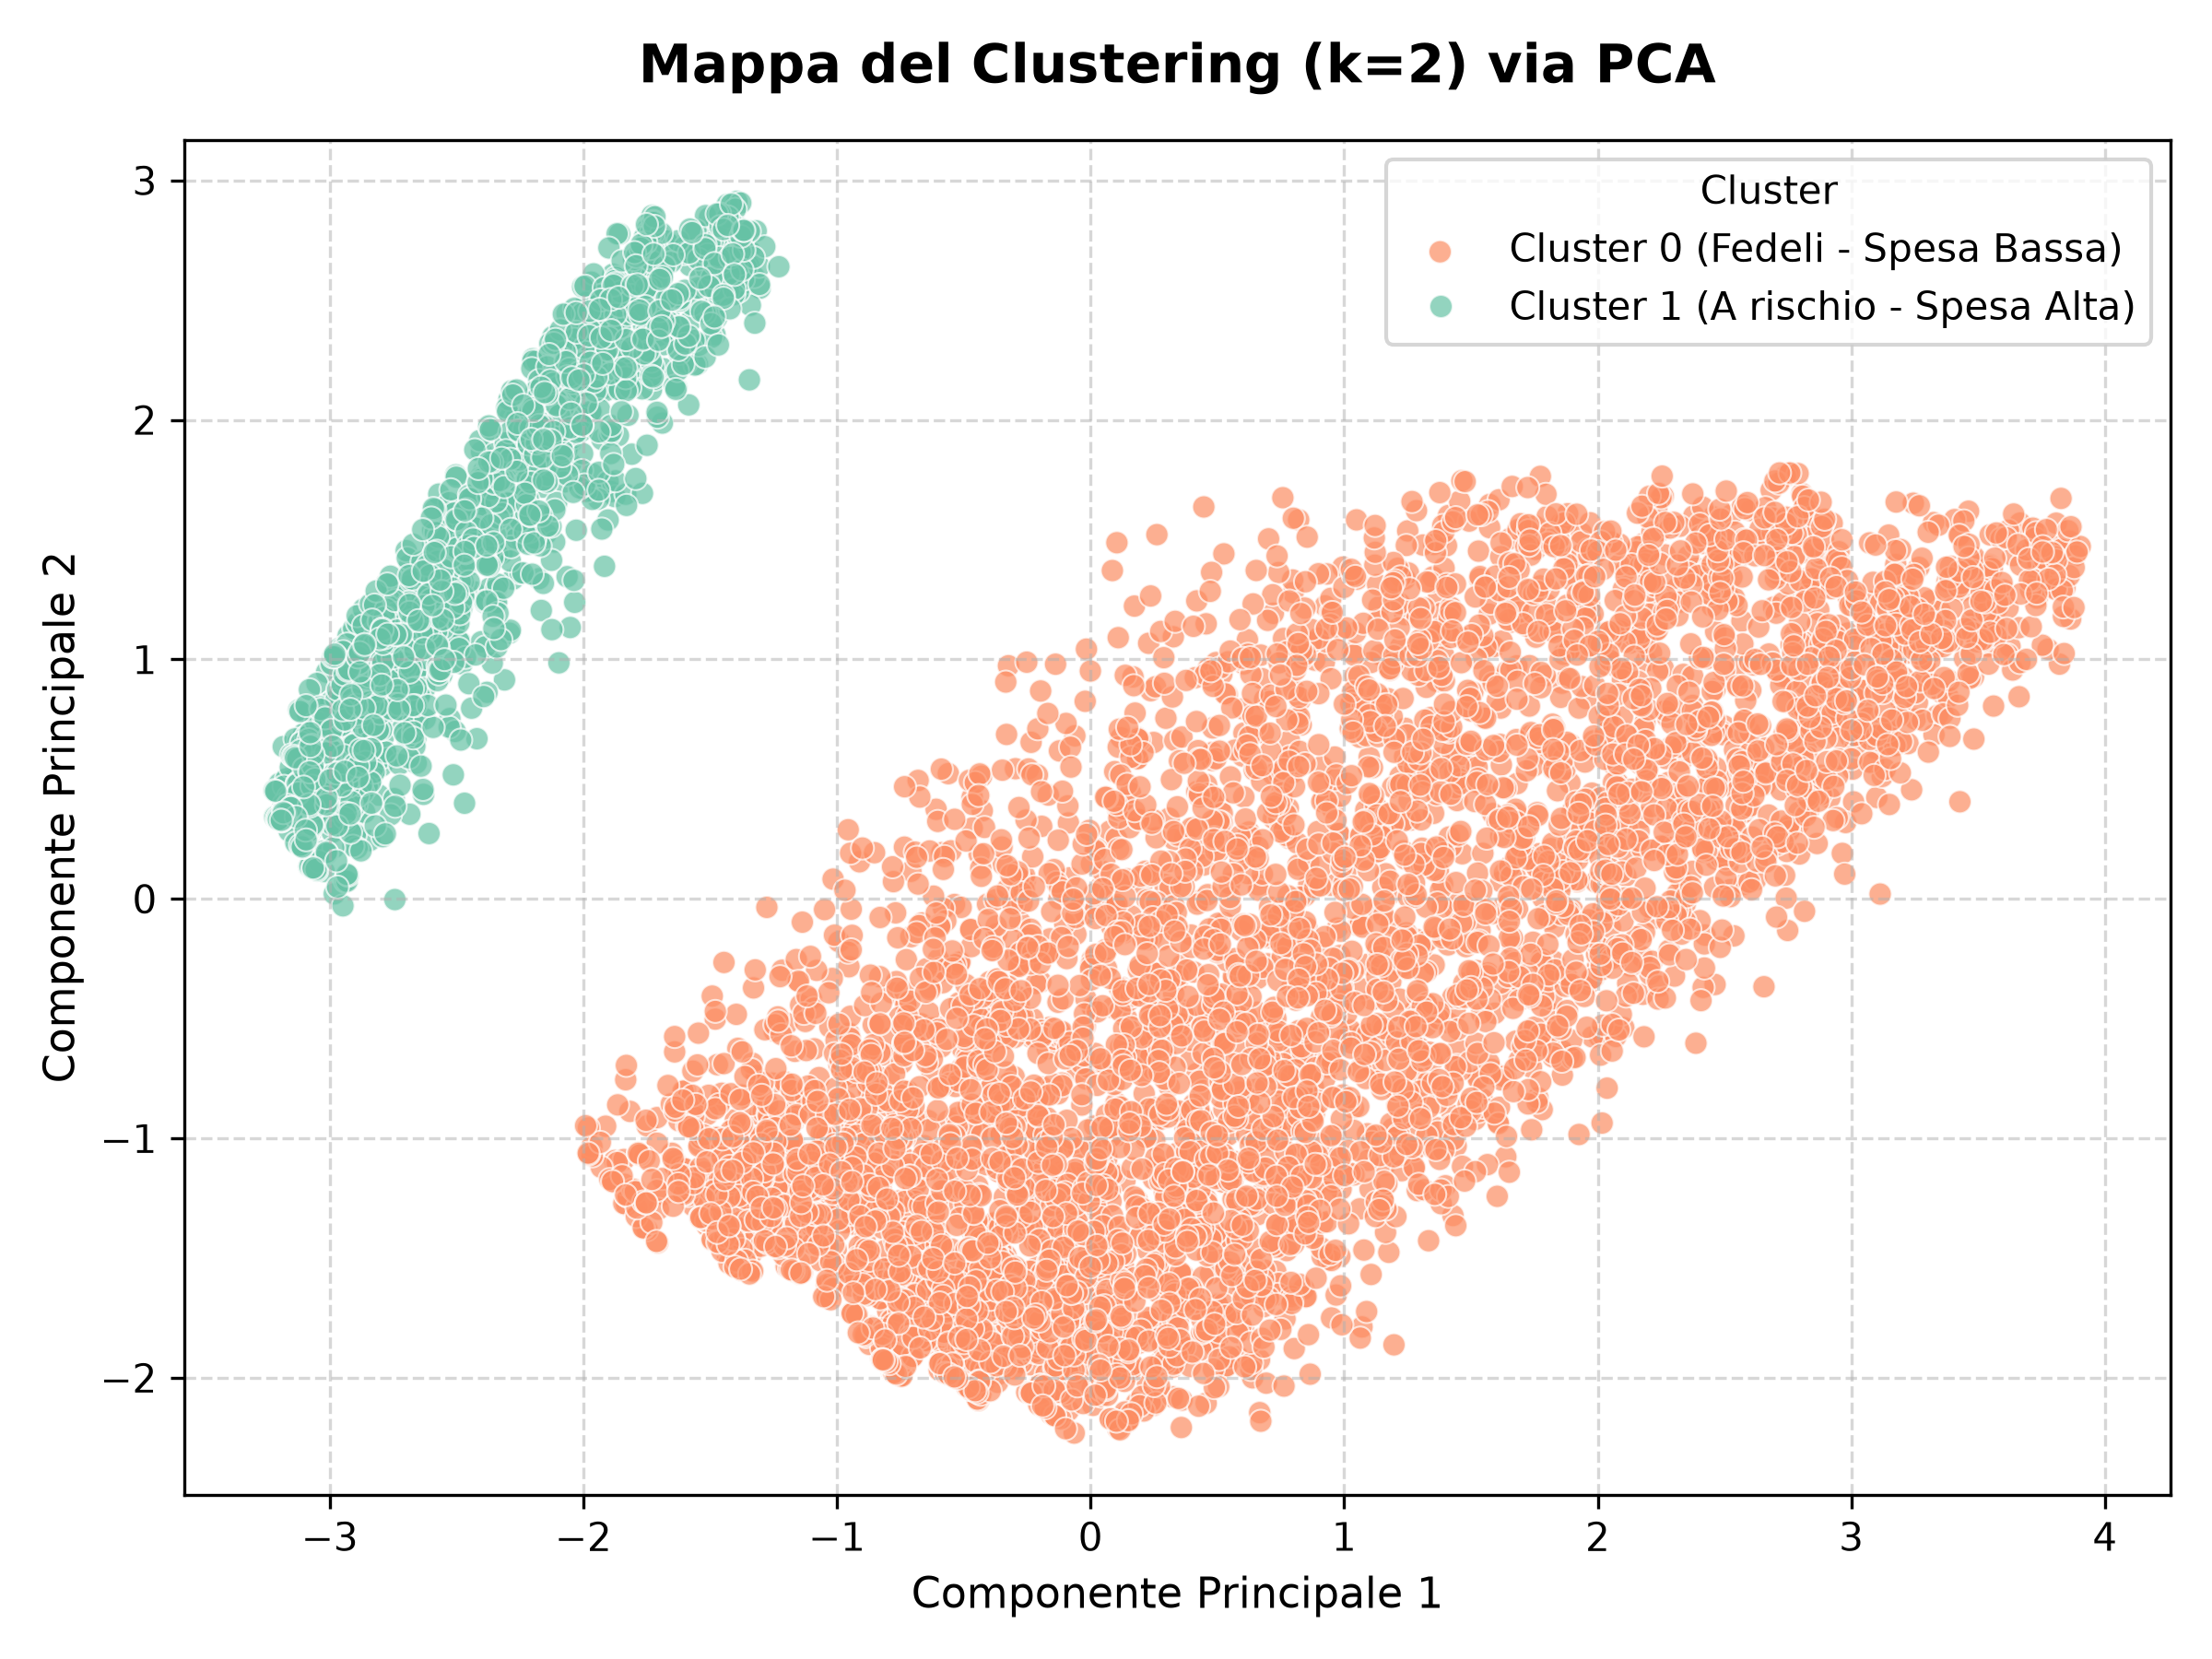
\includegraphics[width=\textwidth]{../grafici/clustering_map.png}
        \caption{Mappa del clustering k-Means ($k=2$) che mostra la distribuzione dei due cluster.}
        \label{fig:clustering_map}
    \end{minipage}
\end{figure}

\subsection{Risultati della Classificazione (Train vs. Test)}
Per predire il Churn ho confrontato tre modelli con filosofie diverse:
\begin{enumerate}
    \item \textbf{Regressione Logistica}: Il modello di baseline lineare, semplice e veloce, che stima la probabilità tramite la funzione sigmoide. Ci serve come base semplice di confronto.
    \item \textbf{Albero di Decisione}: Un modello a regole logiche (IF-THEN), facilmente visualizzabile, che suddivide i clienti in base alle scelte che riducono di più l'impurezza.
    \item \textbf{Multi-Layer Perceptron (MLP)}: Un modello non lineare complesso (rete neurale artificiale) composto da strati di neuroni collegati che apprendono relazioni non lineari grazie alle funzioni di attivazione ReLU e Sigmoide.
\end{enumerate}

Le metriche di performance sono valutate in due scenari sperimentali:
\begin{itemize}
    \item \textbf{Scenario A (Senza Cluster)}: I modelli si addestrano solo sulle caratteristiche preelaborate originarie.
    \item \textbf{Scenario B (Con Cluster)}: Aggiungiamo ai dati il cluster di appartenenza (0 o 1) calcolato da k-Means, per vedere se questa informazione commerciale pre-raggruppata aiuta la predizione.
\end{itemize}

La Tabella \ref{tab:classification_results} riassume le performance su Train e Test.

\begin{table}[htbp]
\centering
\caption{Confronto delle metriche di classificazione tra Train e Test.}
\label{tab:classification_results}
\resizebox{\textwidth}{!}{
\begin{tabular}{llcccccc}
\toprule
 & & \multicolumn{2}{c}{\textbf{Accuracy}} & \multicolumn{2}{c}{\textbf{Recall}} & \multicolumn{2}{c}{\textbf{AUC}} \\
\cmidrule(lr){3-4} \cmidrule(lr){5-6} \cmidrule(lr){7-8}
\textbf{Modello} & \textbf{Feature Scenario} & \textbf{Train} & \textbf{Test} & \textbf{Train} & \textbf{Test} & \textbf{Train} & \textbf{Test} \\
\midrule
Logistic Regression & Senza Cluster & 0.8053 & 0.8062 & 0.5485 & 0.5588 & 0.8492 & 0.8422 \\
Logistic Regression & Con Cluster & 0.8051 & 0.8055 & 0.5485 & 0.5588 & 0.8492 & 0.8423 \\
\midrule
Decision Tree & Senza Cluster & 0.8023 & 0.7942 & 0.5612 & 0.5401 & 0.8476 & 0.8267 \\
Decision Tree & Con Cluster & 0.8023 & 0.7942 & 0.5612 & 0.5401 & 0.8476 & 0.8267 \\
\midrule
Multi-Layer Perceptron (MLP) & Senza Cluster & 0.9143 & 0.7495 & 0.7813 & 0.4278 & 0.9656 & 0.7844 \\
Multi-Layer Perceptron (MLP) & Con Cluster & 0.9104 & 0.7360 & 0.9097 & \textbf{0.5829} & 0.9722 & 0.7846 \\
\bottomrule
\end{tabular}
}
\end{table}

\subsection{Analisi dei Risultati, dell'Overfitting e dell'Impatto delle Feature}
Dall'ispezione della Tabella \ref{tab:classification_results} emergono tre osservazioni fondamentali:
\begin{enumerate}
    \item \textbf{Regressione Logistica e Albero di Decisione sono stabili}: Le loro prestazioni su Train e Test differiscono di pochissimo (accuratezza stabile $\approx 80\%$, AUC $\approx 84\%$). Non c'è alcun segno di underfitting (i modelli catturano bene il segnale dei dati) né di overfitting. L'aggiunta della feature di cluster non ne modifica le prestazioni poiché questi modelli estraggono già le relazioni lineari elementari presenti nei dati.
    \item \textbf{La Rete Neurale (MLP) soffre di forte overfitting}: Nel train set senza cluster la rete raggiunge l'accuratezza del $91.43\%$ e un AUC del $0.9656$, ma sul test set crolla al $74.95\%$ di accuratezza con Recall al $42.78\%$. Trattandosi di un modello molto parametrizzato e flessibile, ha finito per memorizzare il rumore del dataset di addestramento.
    \item \textbf{L'impatto del Cluster sull'MLP}: Nello Scenario B, l'aggiunta del cluster come feature non elimina l'overfitting sul train, ma fa fare un grande balzo in avanti alla \textbf{Recall sul Test set, che sale dal $42.78\%$ al $58.29\%$ ($+15.51\%$ assoluto)}. Questo dimostra che l'informazione commerciale del cluster funge da forte linea guida per l'attivazione dei neuroni della rete, permettendole di scovare molti più clienti a rischio effettivo di abbandono (veri positivi), pur pagando un piccolo costo in termini di falsi positivi (l'accuratezza sul test scende a $73.60\%$).
\end{enumerate}

\subsection{Interpretazione Visiva dei Modelli}

\subsubsection{L'Albero di Decisione Semplificato}
La Figura \ref{fig:decision_tree_vis} mostra le regole logiche dell'albero di decisione. Ciascun nodo contiene la regola di split in alto (se rispettata si scende a sinistra), l'impurezza (\textit{gini}), il numero di campioni (\textit{samples}), la distribuzione delle classi (\textit{value} ovvero \texttt{[No Churn, Churn]}) e la classe di maggioranza (\textit{class}). I nodi sono colorati in \textbf{blu} se prevale No Churn (classe 0) e in \textbf{arancione} se prevale Churn (classe 1). L'intensità del colore indica il grado di purezza.

\subsubsection{Importanza delle Feature}
La Figura \ref{fig:feature_importances} mostra le caratteristiche più importanti per l'albero nello Scenario B: la variabile determinante in assoluto è `Contract\_Month-to-month` (contratto mensile), seguita da `tenure` (mesi di permanenza) e `InternetService\_Fiber optic` (fibra ottica). Nel grafico notiamo che il nostro `Cluster\_1` non compare nella top 10 dell'albero di decisione (in quanto l'albero ricostruisce la logica del cluster tramite split diretti sulle variabili originali). Tuttavia, come visto nella sezione precedente, l'aggiunta del cluster ha un impatto formidabile sulla Rete Neurale (MLP), incrementando la Recall di ben 15.5 punti percentuali.

\begin{figure}[htbp]
    \centering
    \begin{minipage}{0.49\textwidth}
        \centering
        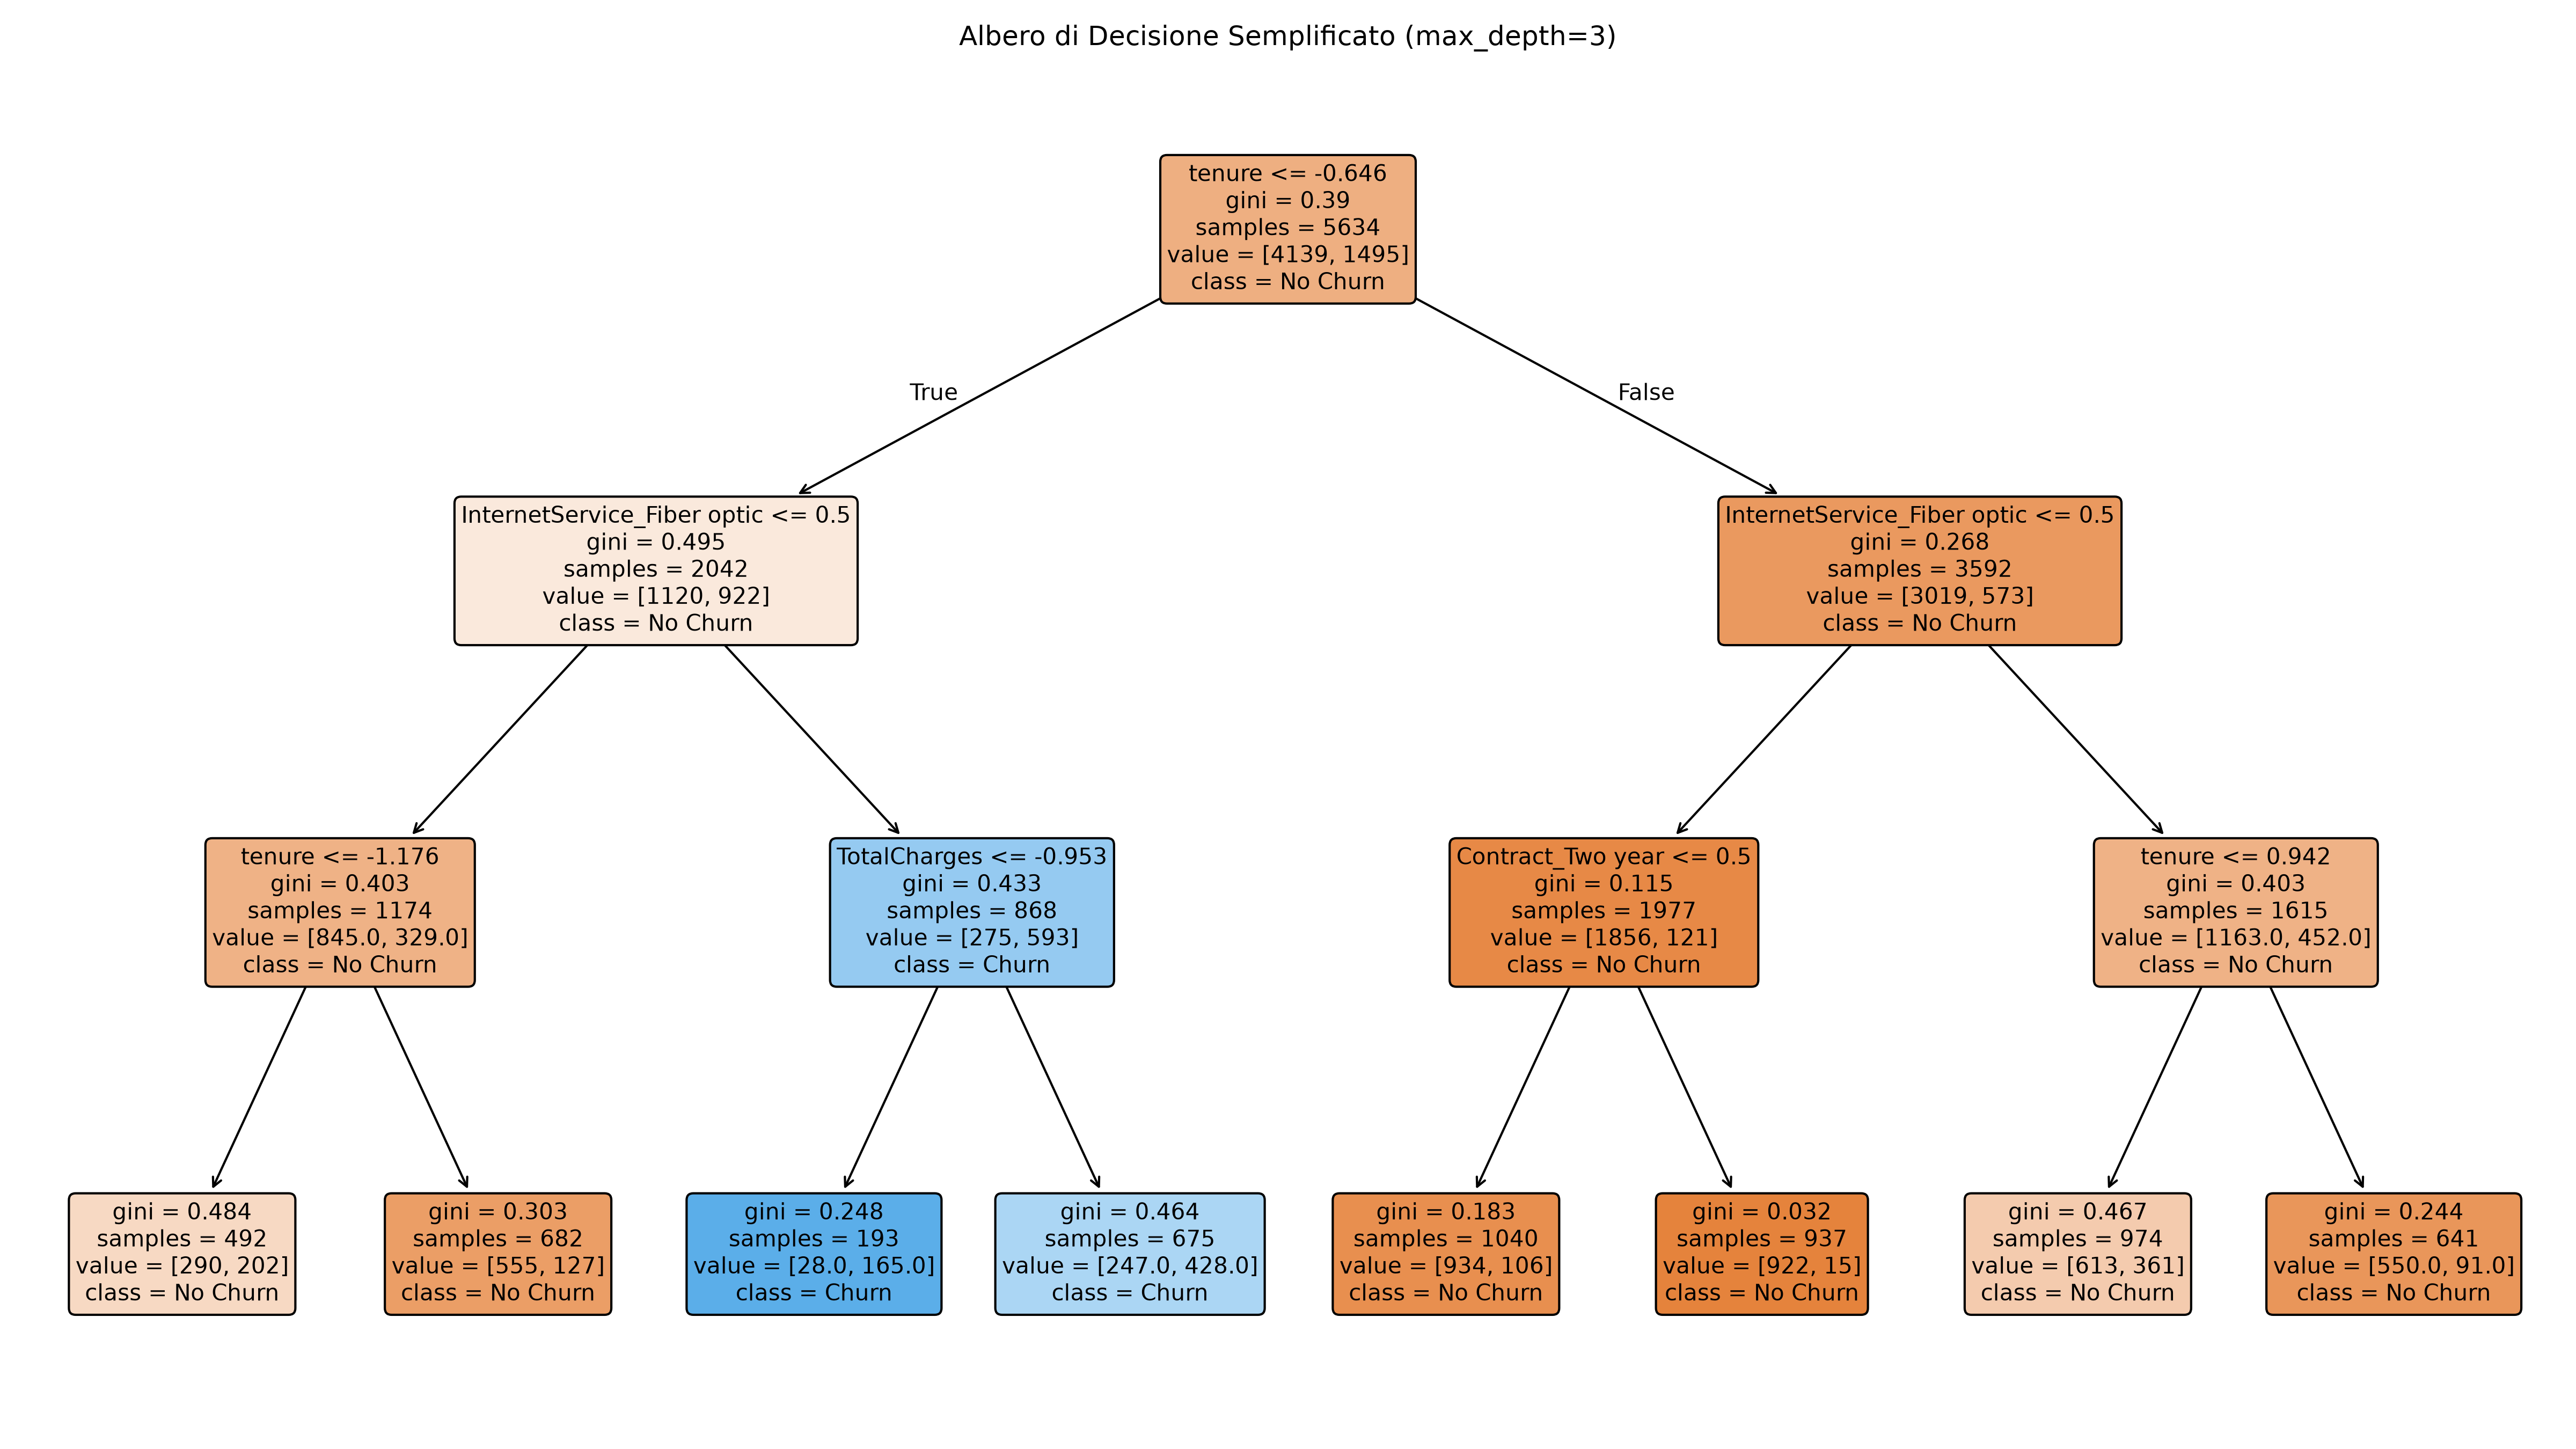
\includegraphics[width=\textwidth]{../grafici/decision_tree_vis.png}
        \caption{Albero di Decisione semplificato ($max\_depth=3$).}
        \label{fig:decision_tree_vis}
    \end{minipage}\hfill
    \begin{minipage}{0.49\textwidth}
        \centering
        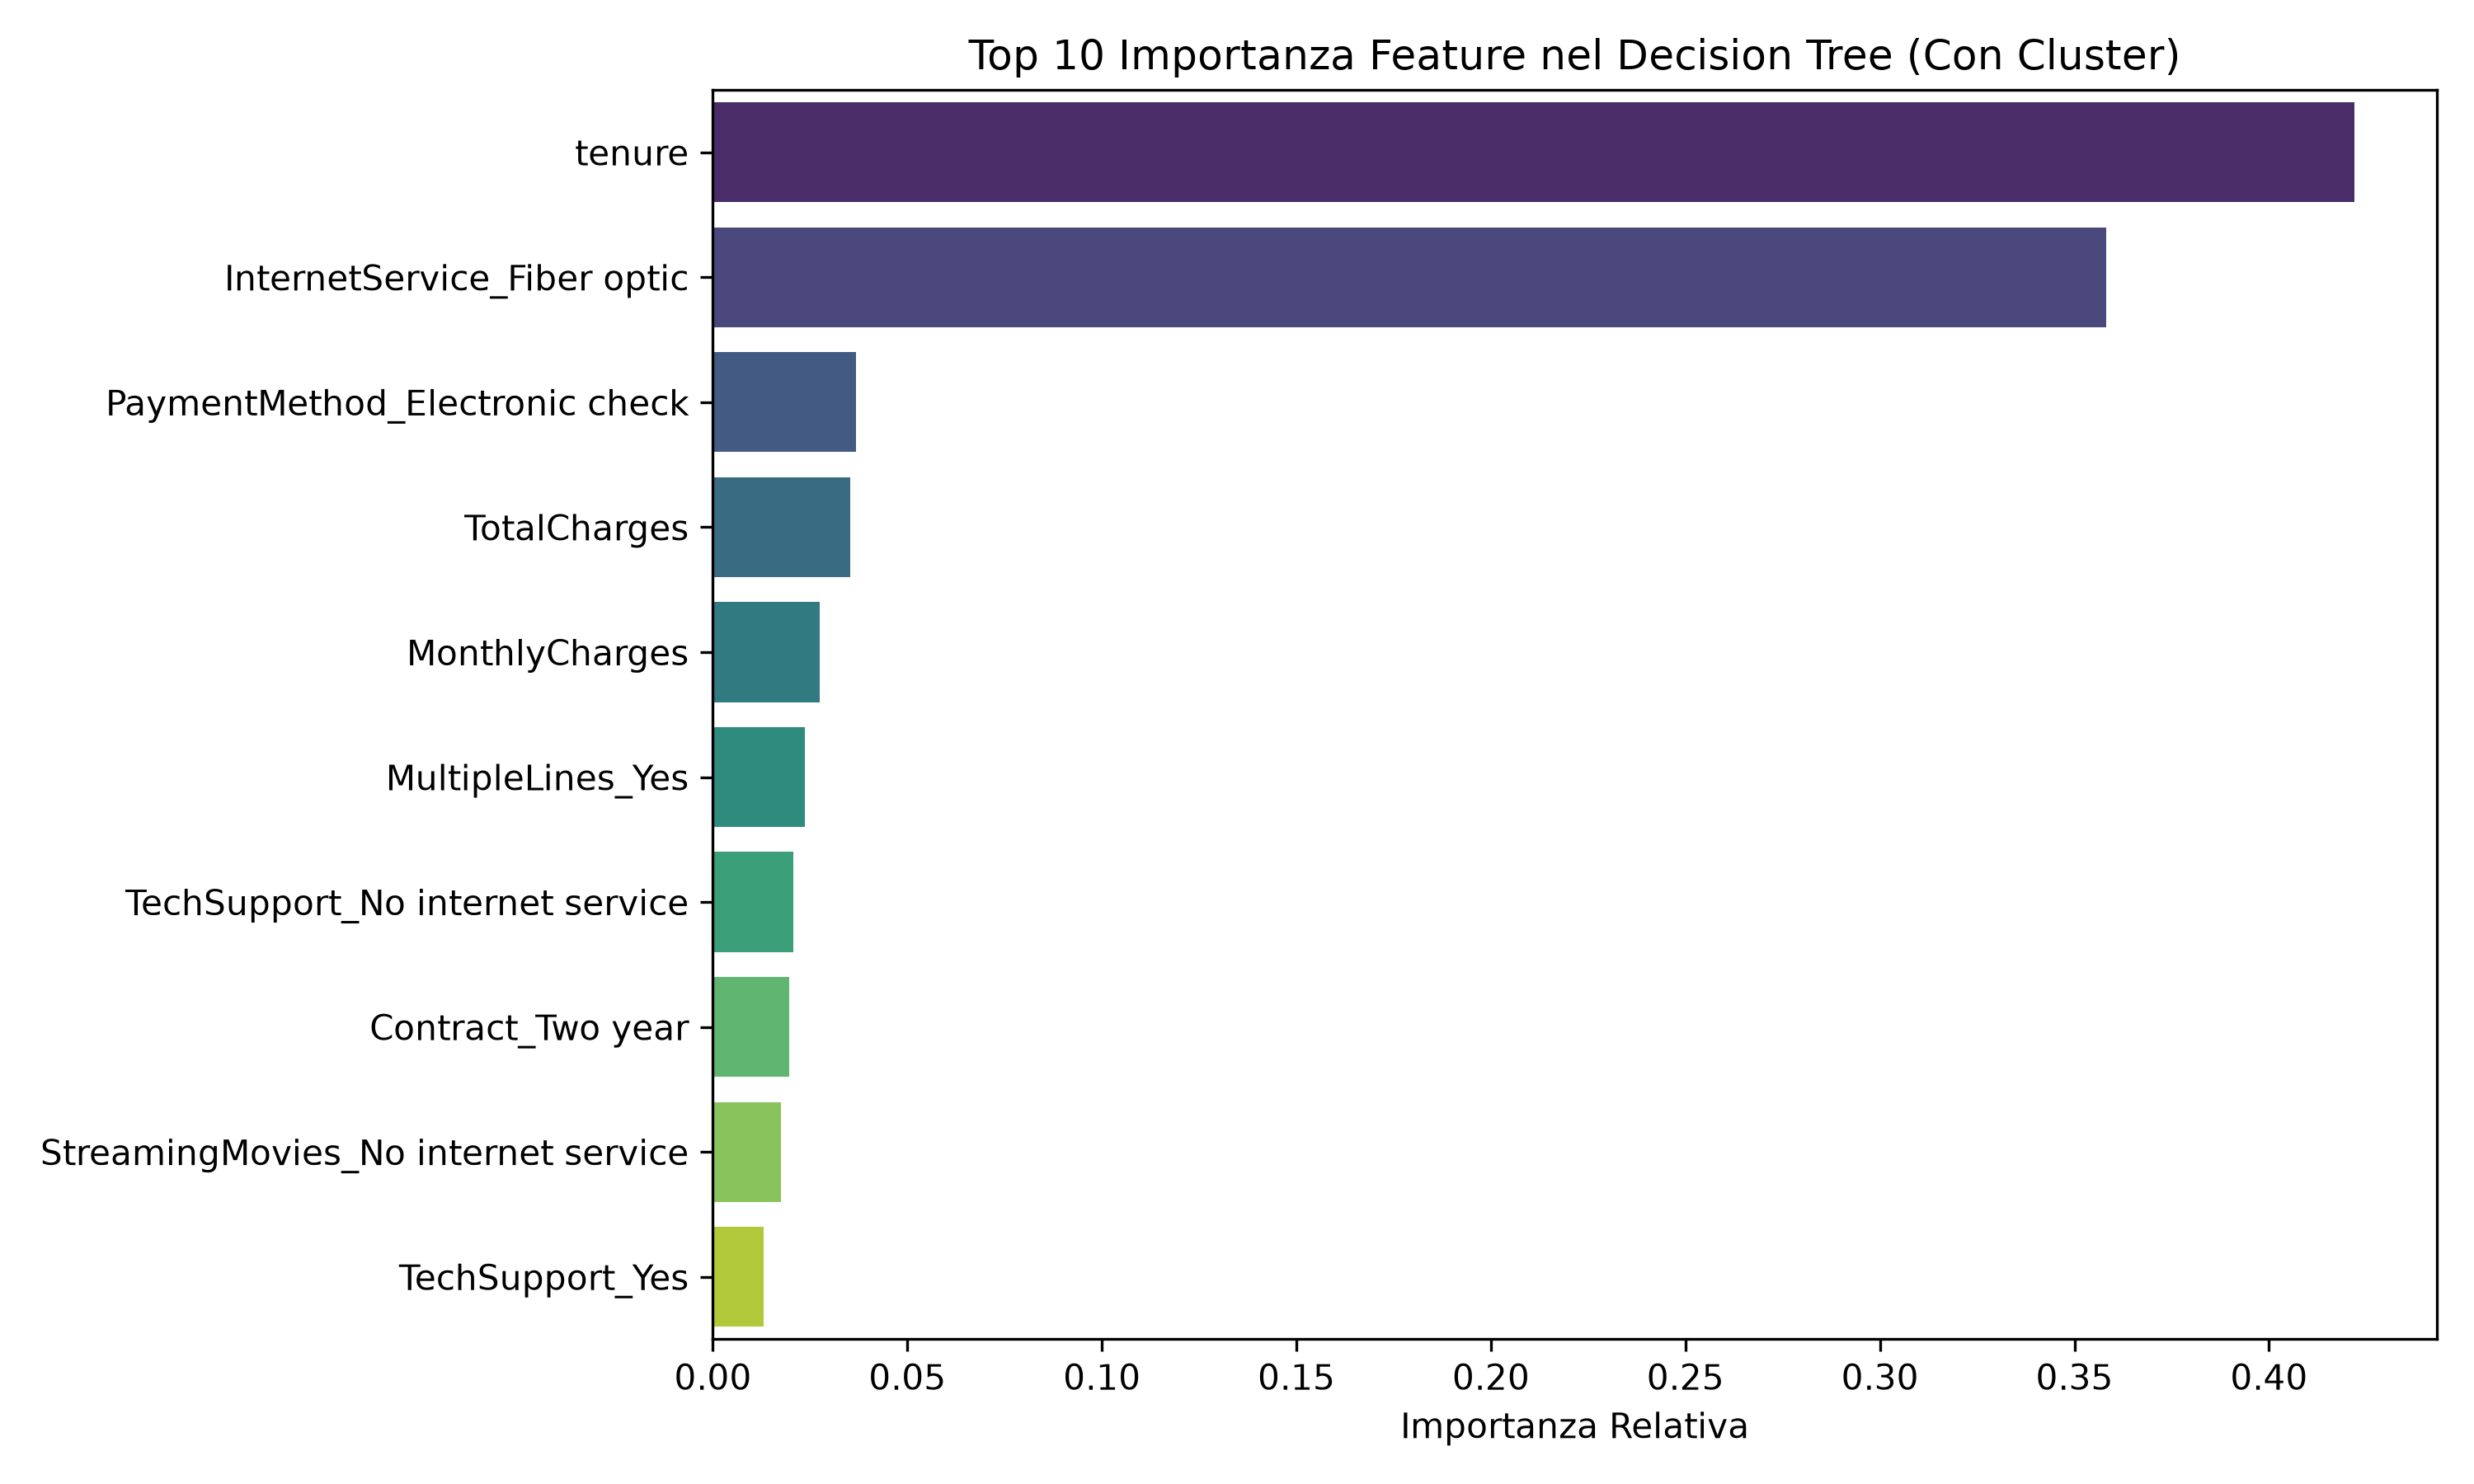
\includegraphics[width=\textwidth]{../grafici/feature_importances.png}
        \caption{Top 10 importanza delle feature nello Scenario B.}
        \label{fig:feature_importances}
    \end{minipage}
\end{figure}

% -------------------------------------------------------------
\section{Discussione critica}
\label{sec:discussione_critica}

\subsection{Punti di Forza della Soluzione}
Unire il clustering non supervisionato e la classificazione ha permesso di descrivere chiaramente i profili commerciali dei clienti. Inoltre, l'aggiunta del cluster come caratteristica ha dato un aiuto concreto alla rete neurale MLP, aumentandone la Recall sul test set di oltre il $15\%$, un risultato molto utile per l'azienda.

\subsection{Limiti Sperimentali e Fonti di Errore}
I due cluster trovati hanno confini un po' sfumati (Silhouette Score di $0.2946$), segno che i clienti non sono divisi in categorie nette ma hanno comportamenti intermedi. Inoltre, il forte overfitting dell'MLP dimostra che la rete neurale così com'è non è pronta per essere usata, e servirebbero tecniche per frenare questa tendenza (come l'aumento della regolarizzazione L2, il dropout o l'Early Stopping).

\subsection{Confronto: Decision Tree vs. MLP}
L'Albero di Decisione è un modello trasparente (\textit{white-box}): guardando la Figura \ref{fig:decision_tree_vis} si capiscono al volo le regole usate per classificare un cliente (la regola più importante è se il contratto è mensile e quanti mesi di permanenza ha il cliente). La Rete Neurale (MLP), invece, è una scatola nera (\textit{black-box}): anche se offre una Recall migliore, è impossibile spiegare a parole come i pesi dei collegamenti arrivino a quella decisione, rendendola difficile da usare se l'azienda vuole capire i motivi precisi dietro le scelte dei clienti.

\subsection{Miglioramenti Futuri}
Per migliorare i modelli proporrei di:
\begin{itemize}
    \item Bilanciare le classi (ad esempio impostando il parametro \texttt{class\_weight='balanced'} nei modelli o ponderando le classi) per gestire lo sbilanciamento del dataset.
    \item Provare modelli ensemble come Random Forest o XGBoost, che spesso gestiscono meglio l'overfitting rispetto alle reti neurali su dati tabellari.
\end{itemize}

\subsection{Uso di strumenti di Intelligenza Artificiale Generativa}
Per lo sviluppo di questo progetto ho utilizzato strumenti di intelligenza artificiale generativa (Large Language Models) solo per farmi aiutare a formattare il codice in \LaTeX\ e a impostare lo scheletro della relazione.

\section{Conclusioni}
\label{sec:conclusioni}
Il progetto ha dimostrato che unire apprendimento non supervisionato e supervisionato è una scelta vincente. Il clustering ha identificato due gruppi commerciali chiari (clienti fedeli che spendono poco contro clienti volatili che spendono molto). Aggiungere questa suddivisione come caratteristica ha aiutato a ridurre l'impatto dello sbilanciamento del dataset sulla Rete Neurale (MLP), portando a un incremento del $+15.5\%$ nel richiamo dei clienti a rischio di abbandono sul Test Set, anche se rimangono aperti i problemi di overfitting della rete che richiederanno modelli più regolarizzati in futuro.

\end{document}
